\documentclass{report}
\usepackage{listings}
\usepackage{hyperref}
\usepackage{tikz}
\usetikzlibrary{shapes.geometric, arrows, positioning}
\tikzstyle{process} = [rectangle, minimum width=3cm, minimum height=1cm, text centered, text width=6cm, draw=black]
\tikzstyle{arrow} = [thick,->,>=stealth]

\begin{document}

\title{Tastydoc: a documentation tool for Dotty using TASTy files}
\author{Bryan Abate
\\\\\small{Supervised by Aleksander Boruch-Gruszecki}}

\maketitle

\begin{abstract}
The current documentation tool (Dottydoc) relies on compiler internals and low-level code. The tool introduced in this work aims to build a program that does not depend on compiler internals but instead uses TASTy files. The latter become output when a Scala program is compiled.

This work also aims at providing a better maintained tool with fewer bugs and more features.

The documentation files are in Markdown instead of the commonly used HTML.
\end{abstract}

\tableofcontents

\chapter{Introduction}

A documentation tool is a program generating information (often in the form of HTML files) about projects. Usually, that tool includes method signatures, user-written documentation, links to other pages of the documentation, etc.
In Dotty, the current tool for generating Scala project documentation is called Dottydoc. The tool introduced here, Tastydoc, aims to improve on Dottydoc and replace it.

Tastydoc uses TASTy files. These files contain information about the source code of a program. They become output when a program is compiled. Tastydoc consumes such files to extract information about the code, making its use completely independent of the compiler.
The tool tries to be as close as possible to the structure proposed in Dottydoc so that it can reuse some portions of its code with minor modifications.

The documentation is often output as HTML files, but here we choose to output Markdown files for reasons detailed further in the report.

The tool was developed with a few goals in mind. First, it should be independent of the compiler, hence the use of TASTy files. It should also produce humanly consumable files, hence the choice of Markdown as an output. Finally, it should have as many features as Dottydoc and be as easily maintainable.

The report is organized in the following structure: First, we will talk about the features of the tool. Then, we will give a high-level and a low-level architectural descriptions. Dottydoc and Tastydoc will then be compared. We will finally talk about the problems encountered during the development and the further work needed.

\chapter{Features}
We will list here the most important features of Tastydoc. For a comparison with Dottydoc features see \autoref{sec:comparison}.

\paragraph{Accessible information}
The tool has knowledge of the full signature of entities; that is, awareness of annotations, modifiers (including scope modifiers), parameters, type parameters, and return types.

For classes, traits, and objects the following are also available (when applicable): members, parents, constructors, known subclasses and companion.
Packages know all their members as long as all corresponding TASTy files are passed as arguments to the tool.

User-written documentation, including individual access to defined @ such as \texttt{@param} (except \texttt{@usecase}). Two syntaxes are supported, which are the old Scaladoc Wiki-style syntax as well as Dottydoc Markdown syntax. Linking to entities (classes, methods, etc.) is possible inside the user documentation in the Wiki-style syntax using the notation like \texttt{[[scala.foo.bar]]}.

\paragraph{TASTy}
The tool relies on consuming TASTy files and is hence independent from the compiler.

\paragraph{Linking}
Tastydoc is able to produce links to types defined outside of the current TASTy files (as well as the one inside the file). This is particularly useful for linking to the types of the parameters and return types, companions, scope modifiers, and parents.

\paragraph{Output}
The tool produces Markdown documentation files that are easy to modify and read.

\chapter{Architecture}
\section{High-level architectural descriptions}
\subsection{TASTy}
TASTy is a data format aimed at serializing compiler information about code. Dotty produces these files for each class, object without companion class or trait, trait and package if it contains something else than classes, traits or objects. Given its nature, TASTy is perfect to extract information.
This is done through the use of the reflect API and the making of a class extending \texttt{TastyConsumer}\footnote{\texttt{scala/tasty/file/TastyConsumer.scala}}.

\subsection{High-level API}
The tool offers an interface that is easy to use (called Representation, see \autoref{sec:representation}) to access all the information about an entity in a comprehensible format for anyone willing to write their own documentation tool without worrying to consume TASTy files.

\subsection{Reuse of Dottydoc intermediate representation}
The intermediate structure (Representation) is similar to Dottydoc \texttt{Entity}\footnote{\texttt{dotty/tools/dottydoc/Entity.scala}} allowing to easily reuse parts of Dottydoc code with only minor modifications. Right now, the tool uses parts of Dottydoc code for parsing user documentation. However, it could produce the same HTML files as Dottydoc without relying on compiler internals. Especially since Dottydoc already has a complex templating mechanism that allows to attach blog posts to documentation and a search engine.

\subsection{Markdown}
Outputting Markdown instead of HTML has several advantages. It is easy to edit by hand, easily previewed, and users can easily add their own texts or files to it. A user could, for example, write a Markdown file and link it in the documentation of a class or do the opposite and link a documentation page in a Markdown file.

Markdown files can easily be uploaded for preview to GitHub or GitLab. In that way, it is very easy to upload documentation files along with the code of a project.

Additionally, a lot of tools are available to consume Markdown files and output other formats such as HTML or PDF, making Markdown a nice intermediate representation. We can then imagine a pipeline like this:
\begin{center}
    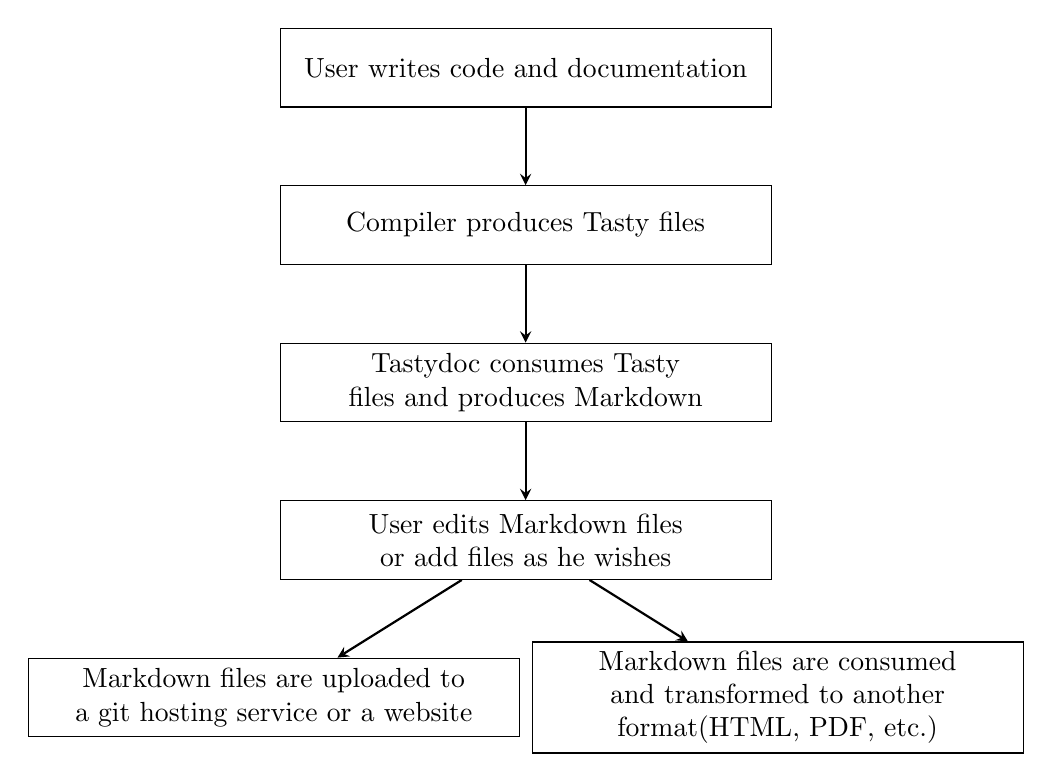
\begin{tikzpicture}[node distance=2cm]
        \node (write) [process] {User writes code and documentation};
        \node (compile) [process, below of=write] {Compiler produces Tasty files};
        \node (tool) [process, below of=compile] {Tastydoc consumes Tasty files and produces Markdown};
        \node (user) [process, below of=tool] {User edits Markdown files or add files as he wishes};
        \node (HTML) [process, below of=user, right of=user, xshift=1.2cm] {Markdown files are consumed and transformed to another format(HTML, PDF, etc.)};
        \node (upload) [process, below of=user, left of=user, xshift=-1.2cm] {Markdown files are uploaded to a git hosting service or a website};
    
        \draw [arrow] (write) -- (compile);
        \draw [arrow] (compile) -- (tool);
        \draw [arrow] (tool) -- (user);
        \draw [arrow] (user) -- (HTML);
        \draw [arrow] (user) -- (upload);
    \end{tikzpicture}
\end{center}

\section{Low-level architecture}
\subsection{TastyExtractor}
File: \texttt{dotty/tastydoc/TastyExtractor.scala}

A trait containing useful methods for extracting information from the reflect API.

\subsection{References}
File: \texttt{dotty/tastydoc/references.scala}

Object containing case classes. References are classes containing information about a specific type to be able to link to its documentation file later on. This is inspired by Dottydoc Reference\footnote{dotty/tools/dottydoc/model/references.scala}. There is a reference for all the existing special types such as "or type". Referencing a user-defined type (such as a class or a type alias) is done using a label (the name of the type, like "String") and a path (the full path in which it is defined, like "/scala/Predef/").

\subsection{TastyTypeConverter}
File: \texttt{dotty/tastydoc/TastyTypeConverter.scala}

Trait containing methods for converting from Reflect types to References.

\subsection{Representation}
\label{sec:representation}
File: \texttt{dotty/tastydoc/representations.scala}

Object implementing both \texttt{TastyExtractor} and \texttt{TastyTypeConverter} and containing classes.

A Representation contains all the information of a specific entity. The logic is as follows: there are different traits such as \texttt{Modifiers} or \texttt{Members} and classes which implement those traits. That logic is inspired by dotty-doc Entities\footnote{\texttt{dotty/tools/dottydoc/Entity.scala}}.

A Representation take a reflect class such as \texttt{reflect.ClassDef} and extract every information from it using mostly \texttt{TastyExtractor} functions while converting types to References using \texttt{TastyTypeConverter} functions.

Representations then can be easily used for printing: their content is self-explanatory and their use requires no knowledge of TASTy as the implementation is not exposed from the outside.

We give below the existing Representation, a quick description and their signature (without parameters).
\begin{itemize}
    \item \texttt{PackageRepresentation} For packages
\begin{lstlisting}[language=scala]
class PackageRepresentation(...)
extends Representation with Members
\end{lstlisting}
    \item \texttt{ImportRepresentation} For imports, never used in the tool
\begin{lstlisting}[language=scala]
class ImportRepresentation(...)
extends Representation
\end{lstlisting}
    \item \texttt{ClassRepresentation} For classes, objects and traits, including case classes and case objects.
\begin{lstlisting}[language=scala]
class ClassRepresentation(...)
extends Representation with Members
with Parents with Modifiers with Companion
with Constructors with TypeParams
\end{lstlisting}
    \item \texttt{DefRepresentation} For defs
\begin{lstlisting}[language=scala]
class DefRepresentation(...)
extends Representation with Modifiers
with TypeParams with MultipleParamList
with ReturnValue
\end{lstlisting}
    \item \texttt{ValRepresentation} For vals and vars
\begin{lstlisting}[language=scala]
class ValRepresentation(...)
extends Representation with Modifiers
with ReturnValue
\end{lstlisting}
    \item \texttt{TypeRepresentation} For type alias
\begin{lstlisting}[language=scala]
class TypeRepresentation(...)
extends Representation with Modifiers
with TypeParams 
\end{lstlisting}
    \item \texttt{EmulatedPackageRepresentation} This Representation allow to regroup every PackageRepresentation of the same package under the same Representation. In fact, Tasty will output a Tasty file for each entity in a package and the top of the \texttt{reflect.Tree} is a \texttt{reflect.PackageClause}. Thus, there will be multiple \texttt{PackageRepresentation} of the same package when converting multiple classes of the same package. That latter point can be problematic in regard to usability. This Representation counters that issue. When using an \texttt{EmulatedPackageRepresentation}, it looks to the user as if he were using a \texttt{PackageRepresentation} containing all the members of the package.
\end{itemize}

\subsection{DocPrinter}
File: \texttt{dotty/tastydoc/DocPrinter.scala}

Object with functions that formats Representations and References to Markdown and writes them to files. Basically, it handles all the formatting and printing logic of the tool.

\subsection{mdscala}
File: \texttt{dotty/tastydoc/mdscala.scala}

Object that has helper functions for outputting markdown. Unfortunately, it does not handle escaping as it is a non-trivial task and would require a significant amount of time (see \autoref{sec:problems}).

\subsection{TastyDocConsumer}
File: \texttt{dotty/tastydoc/TastyDocConsumer.scala}

Extends TastyConsumer and consumes TASTy files to produce Representations. It needs a \texttt{mutable.HashMap[String, EmulatedPackageRepresentation]} as parameters for adding every new seen package to the map. This behaviour is required for two reasons: to link inside user documentation and to have a data structure for storing converted Representations.
\subsection{Main}
File: \texttt{dotty/tastydoc/Main.scala}

Manages the workflow (see \autoref{sec:workflow}).

Command line arguments are:
\begin{itemize}
    \item \textbf{-syntax} \{\textit{wiki} or \textit{markdown}\} Syntax to use for user documentation parsing
    \item \textbf{-packagestolink} \{\textit{regex1 regex2 ...}\} Regexes to specify which packages should be linked when formatting References
    \item \textbf{-classpath} \{\textit{URI}\} Extra classpath for input files
    \item \textbf{-i} \{\textit{file1 file2 ...}\} TASTy files
    \item \textbf{-d} \{\textit{dir1 dir2 ...}\} Directories to recursively find TASTy files
\end{itemize}

\subsection{User documentation parsing}
Files are in the package \texttt{dotty.tastydoc.comment}.

These files are taken from Dottydoc (modified to work with this architecture and output Markdown instead of HTML) and are responsible for parsing user-written documentation.

Note that it uses a library called flexmark-java\footnote{\url{https://github.com/vsch/flexmark-java}} for parsing user documentation written in Markdown.

\section{Workflow}
\label{sec:workflow}
Main workflow is as follows:

\begin{center}
    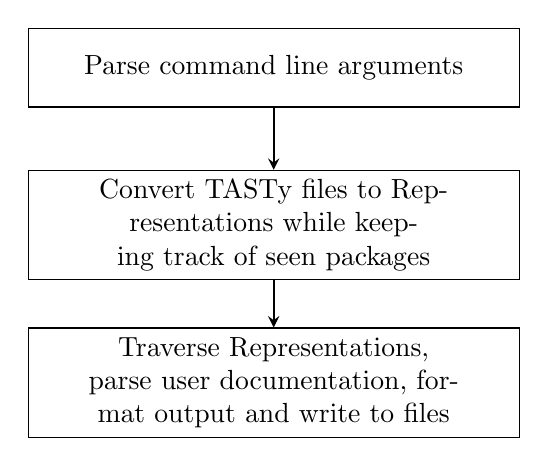
\begin{tikzpicture}[node distance=2cm]
        \node (parse) [process] {Parse command line arguments};
        \node (convert) [process, below of=parse] {Convert TASTy files to Representations while keeping track of seen packages};
        \node (output) [process, below of=convert] {Traverse Representations, parse user documentation, format output and write to files};
    
        \draw [arrow] (parse) -- (convert);
        \draw [arrow] (convert) -- (output);
    \end{tikzpicture}
\end{center}

As we can see, parsing user documentation is only done after converting to Representation. Indeed, in order to link methods, classes, etc. from user documentation we need to have first converted everything to Representation. Otherwise, there is no way to know what is linked (a method? a class? an object?).


\chapter{Comparison between Dottydoc and Tastydoc}
Here we compare Dottydoc and Tastydoc in terms of features, bugs, and output.

\section{General comparison}
\label{sec:comparison}
\paragraph{Compiler internals}
Dottydoc relies on low-level and complex code which makes it very hard to maintain or add features where Tastydoc relies on the comprehensive Reflect API while trying to be as clear and as maintainable as possible. It implies that Tastydoc can be completely moved apart from the compiler and can be distributed as a separate tool.

\paragraph{Output}
Dottydoc outputs HTML/CSS which is not ideal for manual edit and it forces the user to host it on a website where Markdown can simply be viewed on an online git repository without further tasks. Tastydoc counters this problem by outputting Markdown. Also, Markdown can easily be converted to another format.

\section{Extra features from Tastydoc}
\label{sec:extra}
\paragraph{Scope modifiers}
Dottydoc does not handle scope modifiers (such as \texttt{private[this]}) whereas Tastydoc does.

\paragraph{Known subclasses}
Tastydoc keeps track of all seen subclasses of a class and links to their documentation files.

\section{Bugs in Dottydoc that Tastydoc fixes}
Dottydoc is not really maintained and hence does not follow the evolution in Master. Some bugs are present in Dottydoc. Tastydoc fixes them all.

\paragraph{Buggy output}
It does not take care of colors in the \texttt{show} method and it results in faulty type or method output like \texttt{[31m2L[0m}\footnote{\url{https://dotty.epfl.ch/api/dotty/runtime/LazyVals$.html}}.

\paragraph{Wrong parents}
Classes often show to be extending Object instead of their superclass because Object is given first when asking for the parents list to the compiler, example\footnote{\url{https://dotty.epfl.ch/api/scala/Conversion.html}}:
\begin{lstlisting}[language=scala]
    abstract class Conversion [ -T, +U ]
    extends Object with Function1
\end{lstlisting}

\paragraph{Annotations}
Annotations which should not be displayed (like \texttt{@child}) are displayed and sometimes many times\footnote{\url{http://dotty.epfl.ch/api/scala/quoted/Expr.html}}.

\paragraph{Compiler artifacts}
The compiler produces artifacts which should be removed when producing documentation files. For example, default values produce artifacts and Dottydoc does not remove them\footnote{\url{https://dotty.epfl.ch/api/scala/tasty/reflect/Kernel.html}}:
\begin{lstlisting}[language=scala]
    def Definitions_FunctionClass$default$2 : Boolean
\end{lstlisting}

\chapter{Problems}
\label{sec:problems}
A few problems were encountered during the tools' development, some could not be fixed for reasons detailed below.

\paragraph{Markdown escaping}
We need a library to create a Markdown AST and render it to text, because the output is written in Markdown. The library also needs to escape the input. For instance, a method named "\#", will be interpreted as a header of level 1 if it is not escaped which is not the expected behaviour. This creates a problem because no such library exists in Java or Scala and taking care of Markdown escaping would be time-consuming and was not the main topic of this project.

\paragraph{Linking inside code blocks}
We use code blocks indicating we have a piece of code so that a signature is formatted and syntax highlighted. In these code blocks, we also want to be able to make links pointing to the documentation page of a type. Unfortunately, Markdown fenced code blocks do not allow to have links in them. To counter this problem, we use HTML pre and code tag which are also understood by Markdown viewer. However, that causes two problems. First, it is not pure Markdown. Second, we lose the language syntax highlight from Markdown fenced code blocks.

\paragraph{Section}
Markdown does not have "division" with classes like the \texttt{<div>} tag in HTML which could be useful to better structure the page into sections. This is, however, the philosophy of Markdown and is hence an expected feature.

\paragraph{IDs for linking}
If a single entity contains a type and a method definition with the same name (overloaded methods suffer from the same problem), the links we generate do not always point to the correct definition because it links to the first one appearing on the page. This is because most Markdown viewers do not understand user-specified id which could be useful for linking to specific things on the same page. Hence we do not use custom ids for linking in this project and only use automatically generated ids from headers.

To mitigate this problem, we first output types and then values so that when linking it links to the first one appearing in the page which would be a type and it is what we want in most cases. However, this does not solve the problem of linking to type parameters and of linking to overloaded methods.

\chapter{Remaining work}
Although the project is nearly complete, some work needs to be done to perfect the tool.

\paragraph{Markdown escaping}
As seen in \autoref{sec:problems} we do not escape anything before outputting Markdown, this is a problem that needs to be addressed by making a library capable of making a Markdown AST and rendering it to text while escaping the input. This is not a trivial task as Markdown has a lot of different available syntaxes. Especially when we extend Markdown with features such as tables.

\paragraph{Type Lambdas}
Type Lambdas are complex types to handle and convert to References, right now they are converted to constant References. This is not the expected behaviour: the output is not the one we expect and no linking can be done this way. It is, however, acceptable for a first version as type lambdas do not appear that often.

\paragraph{Complex types}
Assume the following type:
\begin{lstlisting}[language=scala]
    class Graph {
        type Node = Int
    }
    def linkingGraph(g: Graph): g.Node = ???    
\end{lstlisting}
Right now the type will only be referenced as \texttt{Node} instead of \texttt{g.Node}.

\paragraph{Default values}
Right now, the tool does not have knowledge of default values for parameters such as \texttt{def(x: Int = 0)} because the way TASTy files keep track of them is complex and not easily accessible.

\paragraph{User-documentation parsing}
User-documentation parsing lacks two features. First, supporting \texttt{@usecase} so that a signature is displayed in the form described in the use case instead of the one in the source code. Second, supporting defined pieces of documentation with \texttt{@define name ...} and then referencing them with \texttt{\$name}\footnote{Example in \url{https://github.com/scala/scala/blob/v2.12.2/src/library/scala/collection/immutable/List.scala\#L73}}.

\paragraph{HTML/CSS}
Markdown files for documentation are good for all the reasons mentioned in this report. However, some people still want a good HTML/CSS documentation. The aim would be to either take back what Dottydoc has and use it with our code or build something new. The first case would be pretty straightforward as our intermediate representation looks very similar to Dottydoc. The biggest modification would be made to the References as links are handled a bit differently in this tool.

\end{document}

%Say that dottydoc does not have these features in problems?
%   Dottydoc no companion, not true?
% Move Md to features from arch?